\documentclass[12pt, dvipsnames, svgnames, x11names,]{article}

\usepackage{xcolor}
% URLs and hyperlinks ---------------------------------------
\usepackage{hyperref}
\hypersetup{
	colorlinks=true,
	linkcolor=NavyBlue,
	filecolor=magenta,      
	urlcolor=blue,
}
\usepackage{xurl}
%---------------------------------------------------
\usepackage[inline]{enumitem}
\usepackage{graphicx}
\usepackage{multirow}
\usepackage{float}
\renewcommand{\arraystretch}{1.40}

% adjust a verrrrry big table -------------------------------
\usepackage{adjustbox}
% -----------------------------------------------------------

\usepackage{array}
% center the p columns and m --------------------------------------------------------------
\newcolumntype{P}[1]{>{\centering\arraybackslash}p{#1}}
\newcolumntype{M}[1]{>{\centering\arraybackslash}m{#1}}
% -------------------------------------------------------------------------------------------------------------

% price
\usepackage{marvosym}
% ----------

\usepackage{xepersian}
\settextfont{Arial}
\setdigitfont{Arial}

\begin{document}
	\begin{titlepage}
		\centering
		\vspace{1cm}
		{\Huge {\textbf{ایندکس معکوس فشرده} \par \lr{Compress Inverted Index}}\par}
		\vspace{15mm}
		\vspace{16mm}
		
\includegraphics[width=11cm]{images/0.jpg} \par
		\vfill \par	\vfill
		\vspace{16mm}
		{\normalsize	سیدمحمدحسین هاشمی  4022363143 \par}
		\vspace{1cm}
		{\large فروردین ۱۴۰3\par}
	\end{titlepage}
	\tableofcontents
	\newpage
	
	
	\section{کلاس \lr{Inverted Index}}
	
		{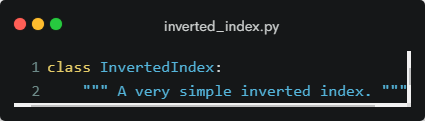
\includegraphics[width=14cm]{images/1.png}}
		\vspace{1cm}
	
		{\normalsize تمام کدهای مربوطه در این کلاس نوشته می‌شود}
	
				
	
	\section{متد \lr{--init--}}
	
		{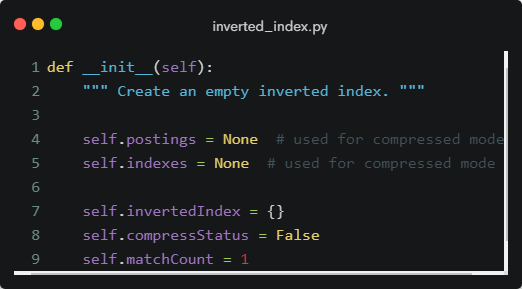
\includegraphics[width=14cm]{images/2.png}} \par
		\vspace{0.5cm}
		{\normalsize
			 در اینجا یک دیکشنری خالی برای ذخیره ایندکس‌های معکوس، دو متغیر \lr{postings}و \lr{indexes} برای حالت فشرده و همچنین وضعیت فشرده بودن و یا نبود را در \lr{compressStatus} ذخیره و در نهایت تعداد کلمات مشابه برای فشرده سازی را در \lr{matchCount} ذخیره می‌کنیم.
			 }
	
	
	\section{متد \lr{read-from-file}}
	
		{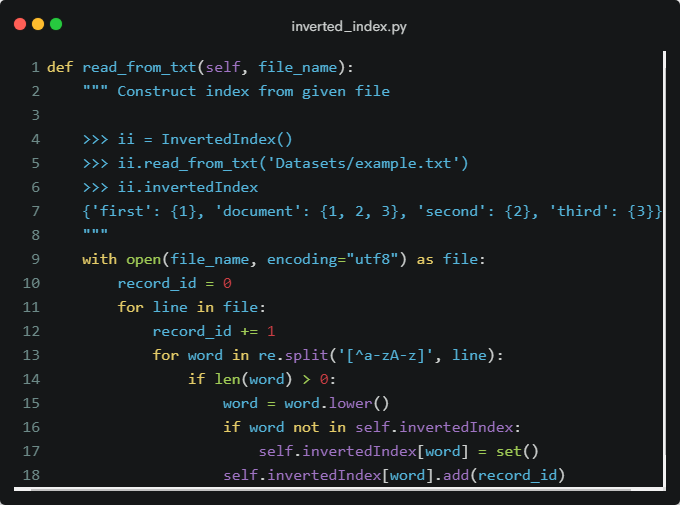
\includegraphics[width=14cm]{images/3.png}} \par
		\vspace{0.5cm}
		{\normalsize
			در این متد فایل حاوی متون دریافت و خوانده می‌شود و لازم به ذکر است که تمامی متحوا درون یک خط قرار می‌گیرد.
		} \par

	
	
	\section{متد \lr{-compress}}
	
		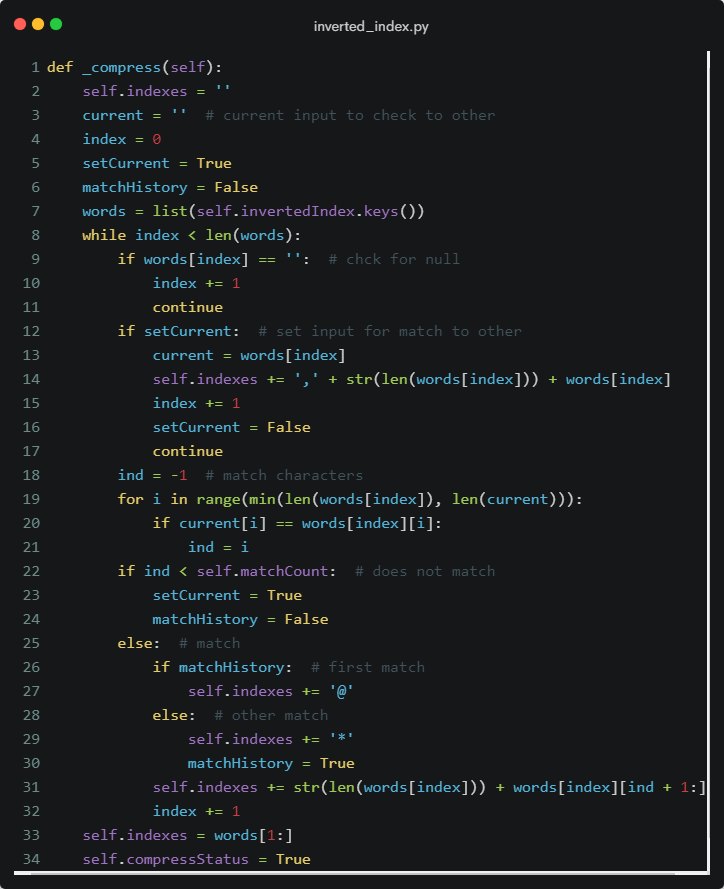
\includegraphics[width=14cm]{images/4.png} \par
		\vspace{0.2cm}
		{\normalsize 
			در این متد ایندکس‌های معکوس را به روش \lr{front-coding} فشرده سازی می‌کنیم.
		}
		
	
	
	\section{متد \lr{extract-d-w}}
		
		\begin{center}
			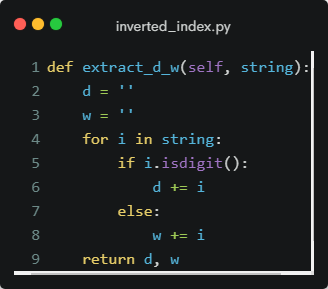
\includegraphics[width=6cm]{images/5.png} \par
		\end{center}
		
		\vspace{0.5cm}
		{\normalsize 
			در این متد کلمه و عدد را در رشته جداسازی می‌کنیم که در متد \lr{-decopress} استفاده می‌شود.
		}		
		
		
	\section{متد \lr{-decompress}}
		
		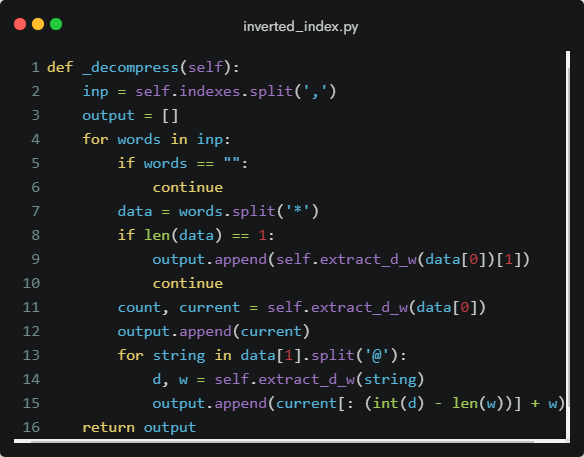
\includegraphics[width=14cm]{images/6.png} \par
		\vspace{0.5cm}
		{\normalsize 
			این متد عکس متد \lr{compress}  عمل کرده و ایندکس‌ها را بصورت یک لیست برمی‌گرداند.
		}		
		
		
	\section{متد \lr{read-from-file}}
		
		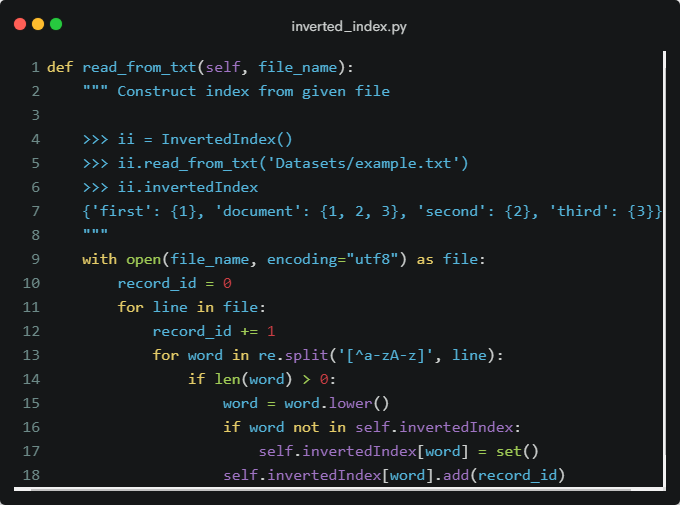
\includegraphics[width=14cm]{images/7.png} \par
		\vspace{0.5cm}
		{\normalsize 
		در این متد فایل حاوی متون دریافت و خوانده می‌شود و لازم به ذکر است که تمامی متحوا درون یک خط قرار می‌گیرد.
		}		
		
		
	\section{متد \lr{compress}}
		
		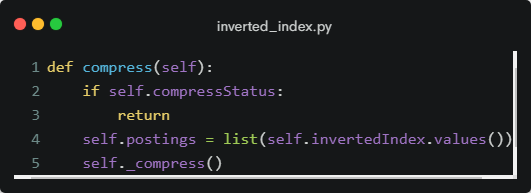
\includegraphics[width=14cm]{images/8.png} \par
		\vspace{0.5cm}
		{\normalsize 
			این متد به قولی \lr{handler} برای متد \lr{-compress}است. که لیست \LR{postings} را جدا می‌کند.
		}		
		
		
	\section{متد \lr{search}}
		
		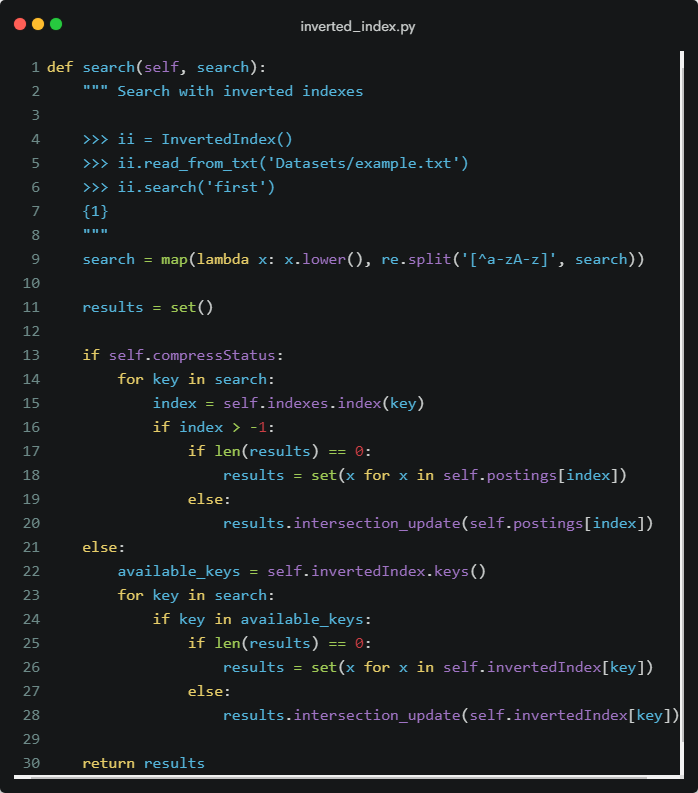
\includegraphics[width=14cm]{images/9.png} \par
		\vspace{0.5cm}
		{\normalsize 
		در این متد عملیات جست‌وجو انجام می‌شود اما این جست‌وجو در دو حالت فشرده نشده و فشرده شده انجام می‌شود که هدف آن مقایسه دو حالت فشرده شده و غیر فشرده است.
		}		
		
		
	\section{خروجی}
		
		\begin{center}
			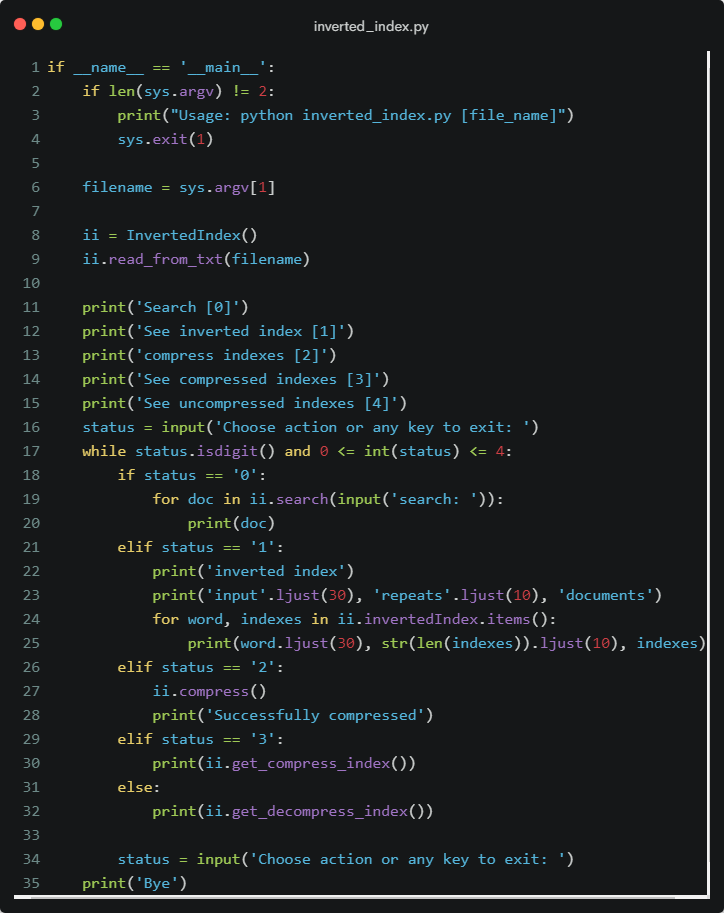
\includegraphics[width=12cm]{images/10.png} \par
		\end{center}
		\vspace{0.1cm}
		{\normalsize 
		همانطور که مشاهده می‌شود ترمینال ساده‌ای جهت کارکردن با برنامه ایجاد شده است. نکته مهم این است که برای دیدن نسخه فشرده ابتدا باید فرمان فشرده سازی اعمال شود و همچنین با این کار جست‌وجو با استفاده از ایندکس‌های فشرده انجام می‌شود.
		}		

	
\end{document}